

\begin{frame}{Bonnes pratiques dans le numérique}{Conseils 60-61/115}
\begin{block}{Favoriser HSTS Preload list aux redirections 301}
Le HSTS indique à n’importe quel navigateur, via un header de réponse HTTP gardé en cache que le domaine doit exclusivement être contacté en HTTPS.
\begin{figure}
    \centering
    
\includegraphics[scale=0.45]{chapitre2/wdd6/fig/c1.png}
\end{figure}
\end{block}

\begin{block}{Mettre en place un plan de fin de vie du site}
\begin{itemize}
    \item Libérer les ressources : décommissionner le service, ses dépendances, les outils utilisés par l’équipe de développement (ex : chanel Teams).
    \item Supprimer, archiver… les données (y compris la GED et le système de suivi des bugs).
    \item Réaffecter les installations, équipements et autres ressources du projet (y compris le code source).
    \item Valoriser les compétences acquises pendant la vie du projet.
\end{itemize}
\end{block}

\end{frame}


\begin{frame}{Bonnes pratiques dans le numérique}{Conseils 62-63/115}
\begin{block}{Choisir un hébergeur écoresponsable}
\begin{enumerate}
    \item gestion des DEEE (déchets d’équipements électriques et électroniques) 
    \item efficience énergétique du data center [Power Usage Effectiveness (PUE) / Carbon Usage Effectiveness (CUE) / Water Usage Effectiveness (WUE)] 
    \item politique d’achat responsable
    \item respect de la dimension sociale
    \item alimentation aux énergies bas carbone
    \item compensation carbone
\end{enumerate}
 \textbf{Exemples :}   OVH,
    SCALEWAY,
    INFOMANIAK

\end{block}

\begin{block}{Privilégier un fournisseur d'électricité écoresponsable}
Utiliser autant que possible une électricité ayant le minimum d'impacts environnementaux lors de sa production 
\end{block}
\end{frame}


\begin{frame}{Bonnes pratiques dans le numérique}{Conseils 64-66/115}
\begin{block}{Adapter la qualité de service et le niveau de disponibilité}
La QoS et le SLA déterminés avec les utilisateurs du site web ou du service en ligne. Inutile d’héberger le service dans un centre de données très haute disponibilité (Tier IV).
\end{block}

\begin{block}{Utiliser des serveurs virtualisés}
Réduire la quantité de déchets électroniques (DEEE) et la consommation électrique.
\begin{itemize}
    \item Utiliser des outils de virtualisation tels que VMware, Xen, KVM, etc.
    \item Utiliser des outils de conteneurisation tels que Docker, Kubernetes, etc.
\end{itemize}
\end{block}

\begin{block}{Optimiser l'efficacité énergétique des serveurs} 
Privilégier des serveurs équipés d’une alimentation électrique conforme à l’écolabel 80Plus (niveaux Platinum et Titanium).

Préférer également les serveurs estampillés Energy Star.
\end{block}

\end{frame}



\begin{frame}{Bonnes pratiques dans le numérique}{Conseils 67-69/115}
\begin{block}{Installer le minimum requis sur le serveur}
Privilégier une installation "manuelle" du serveur (LAMP + CMS, par exemple) plutôt qu’une distribution avec une surcouche de type cPanel ou Plesk.

Et si une surcouche d’administration est nécessaire, préférer des solutions légères comme Webmin.
\end{block}

\begin{block}{Mettre les caches entièrement en RAM (opcode et kvs)}
Les systèmes de cache doivent être montés entièrement en mémoire vive (RAM). 
\end{block}

\begin{block}{Stocker les données dans le cloud}
Pour ne pas multiplier les domaines (conseil n° 55), le plus simple est de regrouper toutes les ressources statiques sur un seul service de stockage en ligne.
\end{block}



\end{frame}


\begin{frame}{Bonnes pratiques dans le numérique}{Conseils 70-71/115}

\begin{block}{Héberger les ressources (CSS/JS) sur un domaine sans cookie}
Les leaders du Web utilisent un domaine séparé pour servir les ressources statiques qui ne nécessitent pas de cookies. Yahoo! emploie le domaine yimg.com, YouTube le domaine ytimg.com et Amazon le domaine images-amazon.com.
\end{block}

\begin{block}{Éviter les redirections}
Les redirections dégradent le temps de réponse, tout en consommant des ressources inutilement. Il faut donc les éviter autant que possible. Ces redirections peuvent avoir lieu à différents niveaux : code HTML, code JavaScript, serveur HTTP et serveur d’applications (PHP, etc.).
\begin{figure}
    \centering
    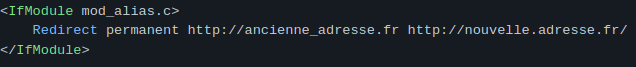
\includegraphics[scale=0.4]{chapitre2/wdd6/fig/c2.png}
\end{figure}
\end{block}

\end{frame}


\begin{frame}{Pause débunkage }{Parlons déchets}
\begin{figure}
    \centering
    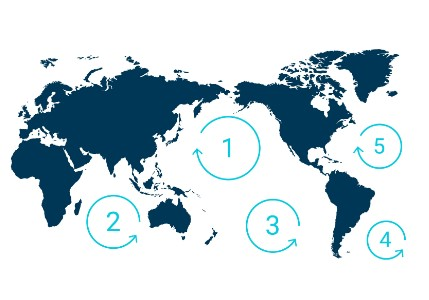
\includegraphics[scale=0.85]{chapitre2/wdd6/fig/carte.jpg}
\end{figure}
\end{frame}